\chapter [Basic Signal Operations]{Basic Signal Operations}


\section{AIM}
\begin{enumerate}
\item
For a given signal generate its
\begin{itemize}
\item
Folded signal sequence
\item
Time delayed and advanced sequences

\end{itemize}
\item
For the given two signals in discrete domain perform signal addition and subtraction
\item
Perform linear convolution on given two sequences..

\end{enumerate}
\section{THEORY}
\paragraph{}

The time reversal of a discrete time signal $x(n)$ can be obtained by folding the sequence about $n=0$ and the folded sequence is represented by $x(-n)$. The signal time delayed by 3 samples  is obtained by shifting the sequence to right by 3 samples and it is represented with $x(n-3)$. The signal time advanced by 2 samples  is obtained by shifting the sequence to left by 2 samples and it is represented with $x(n+2)$.	
	
	
	For discrete-time signals the sum of two sequences and difference of two sequences is obtained by adding and subtracting the sequence values at the same index $n$ for which the sequences are defined.
	
The convolution between the input sequence $x(n)$ and impulse response $h(n)$ is computed using the function $convol$ as $y=convol(x,h)$. If the length of $x(n)$ is $N_1$ and length of $h(n)$ is $N_2$ , then the length of $y(n)$ is $N_1+N_2-1$. The length of $x(n)$ and $h(n)$ is found using the function $length(x)$ and $length(h)$ . If the sequence $x(n)$ is starting at $n_1$ and $h(n)$ at $n_2$, then sequence $y(n)$ starts at $n_1+n_2$.

\section{PROCEDURE}

\paragraph{}
\begin{enumerate}
\item
Start Scilab on PC and Scilab console window opens. Create a new blank SciNote.
\item
The code for the required program is typed and saved as Scilab SCE file with an extension .sci
\item

The continuous plots are made using the function $plot$ and discrete plots are made using the function $plot2d3$ with the corresponding x axis and y axis variables written inside parathesis.

\item
To view all the plots in the same window the function $subplot$ is used.
\item
The results and the errors in the program are displayed in the console window.
The typed program is run using the $execute$.
\item
The resultant figure is exported as pdf using $xs2pdf$
\end{enumerate}

\section{SCILAB CODE}

\lstinputlisting[caption=Scilab code for a folded sequence]{./scilabCode/folded_sequence.sci}

\lstinputlisting[caption=Scilab code for sequences with time shifted versions]{./scilabCode/timeshift.sci}



\lstinputlisting[caption=Addition and Subtraction of signals]{./scilabCode/add_subtract.sci}



\lstinputlisting[caption=Linear Convolution]{./scilabCode/linearconvolution.sci}




\section{RESULT}
Different signal operations were performed using SCILAB.
\begin{figure}
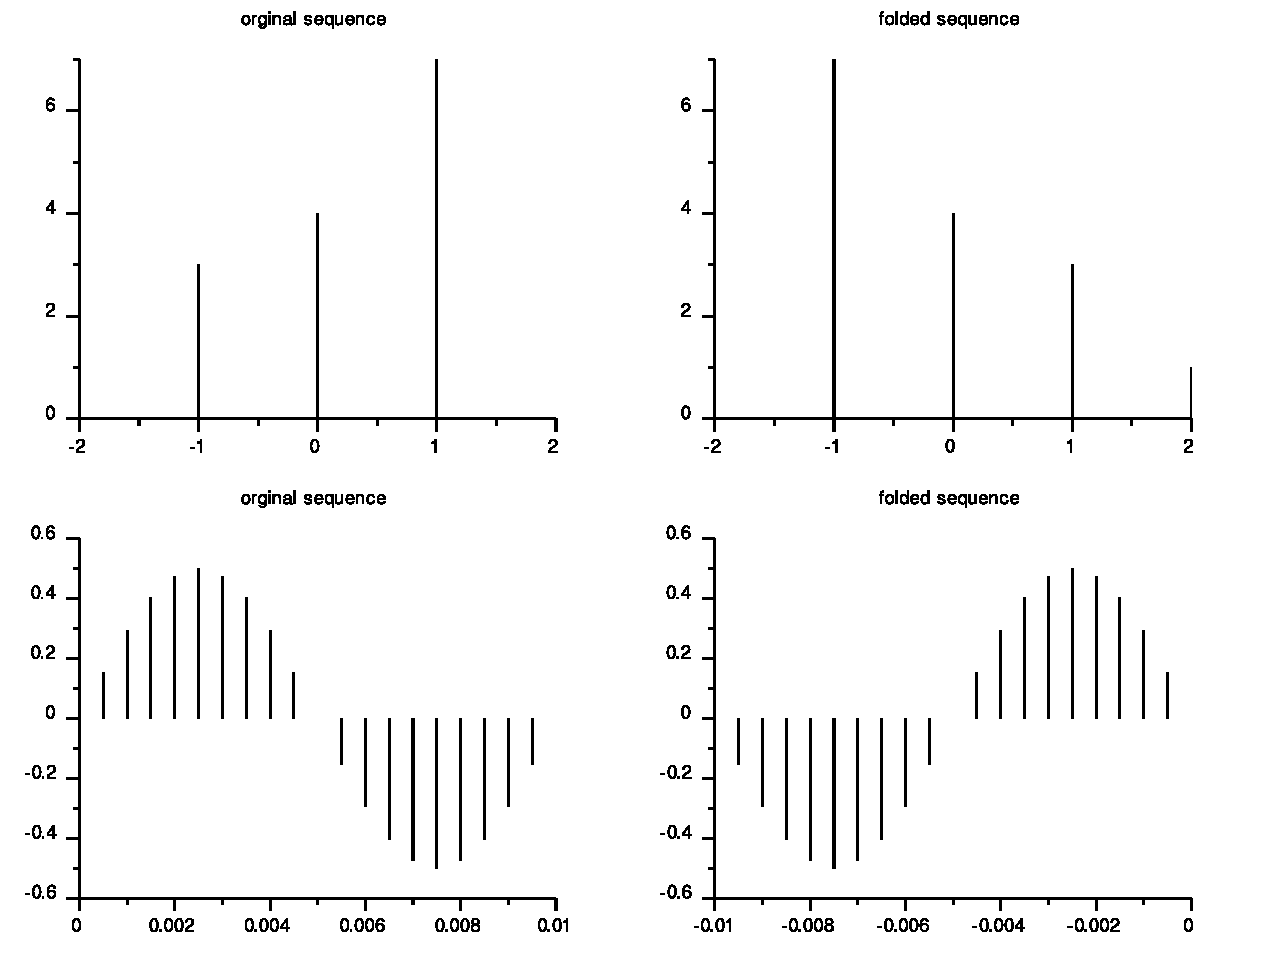
\includegraphics[scale=.5]{/home/kavya/kavyadev/DSPlab/scilabCode/foldedsequence.pdf}
\caption{Plot of signals and their folded versions}
\label{folded}
\end{figure}

\begin{figure}
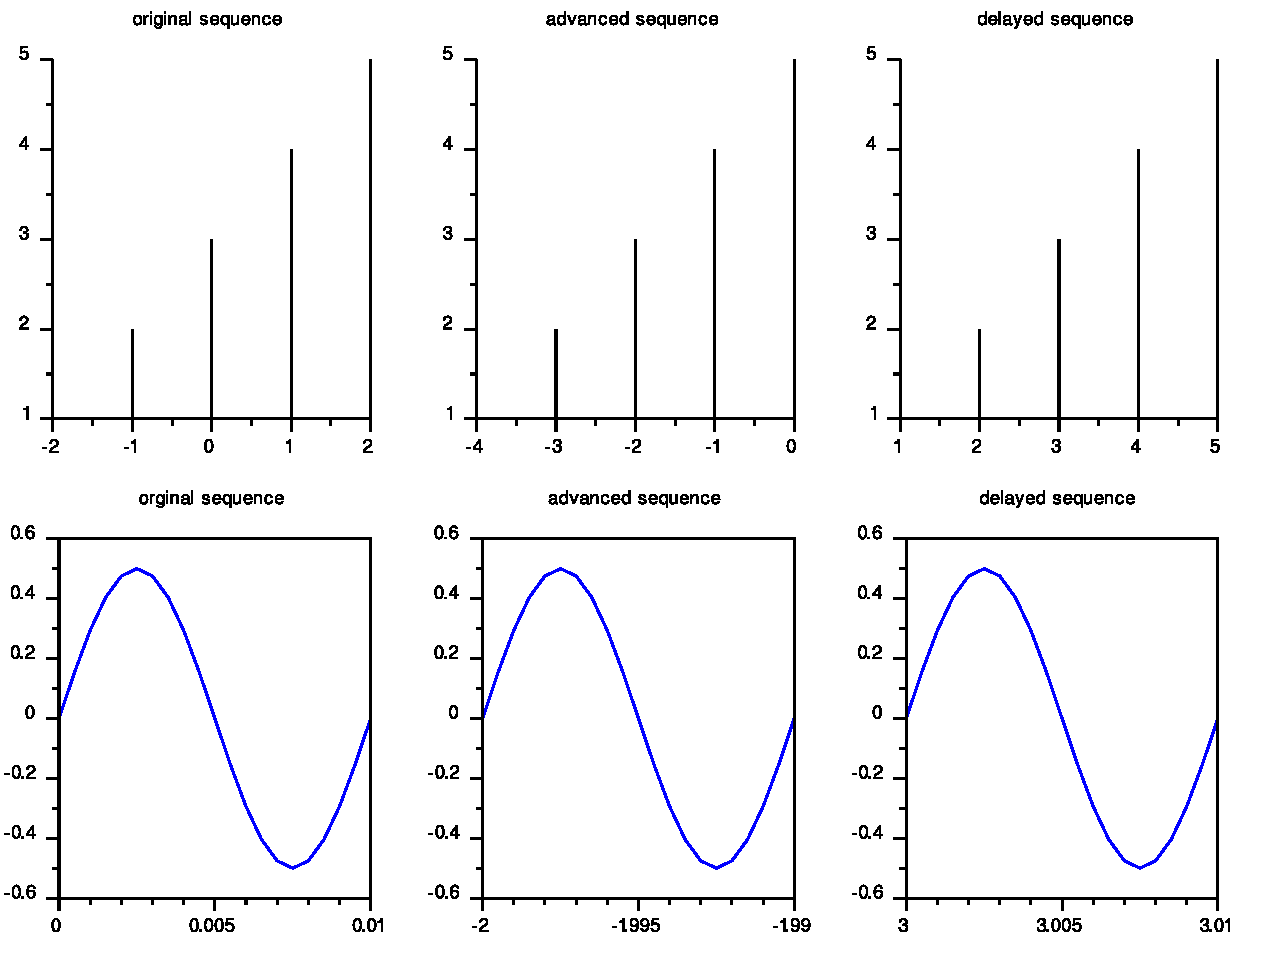
\includegraphics[scale=.5]{/home/kavya/kavyadev/DSPlab/scilabCode/timeshift.pdf}
\caption{Plot of signals and their shifted versions}
\label{shifted}
\end{figure}


\begin{figure}
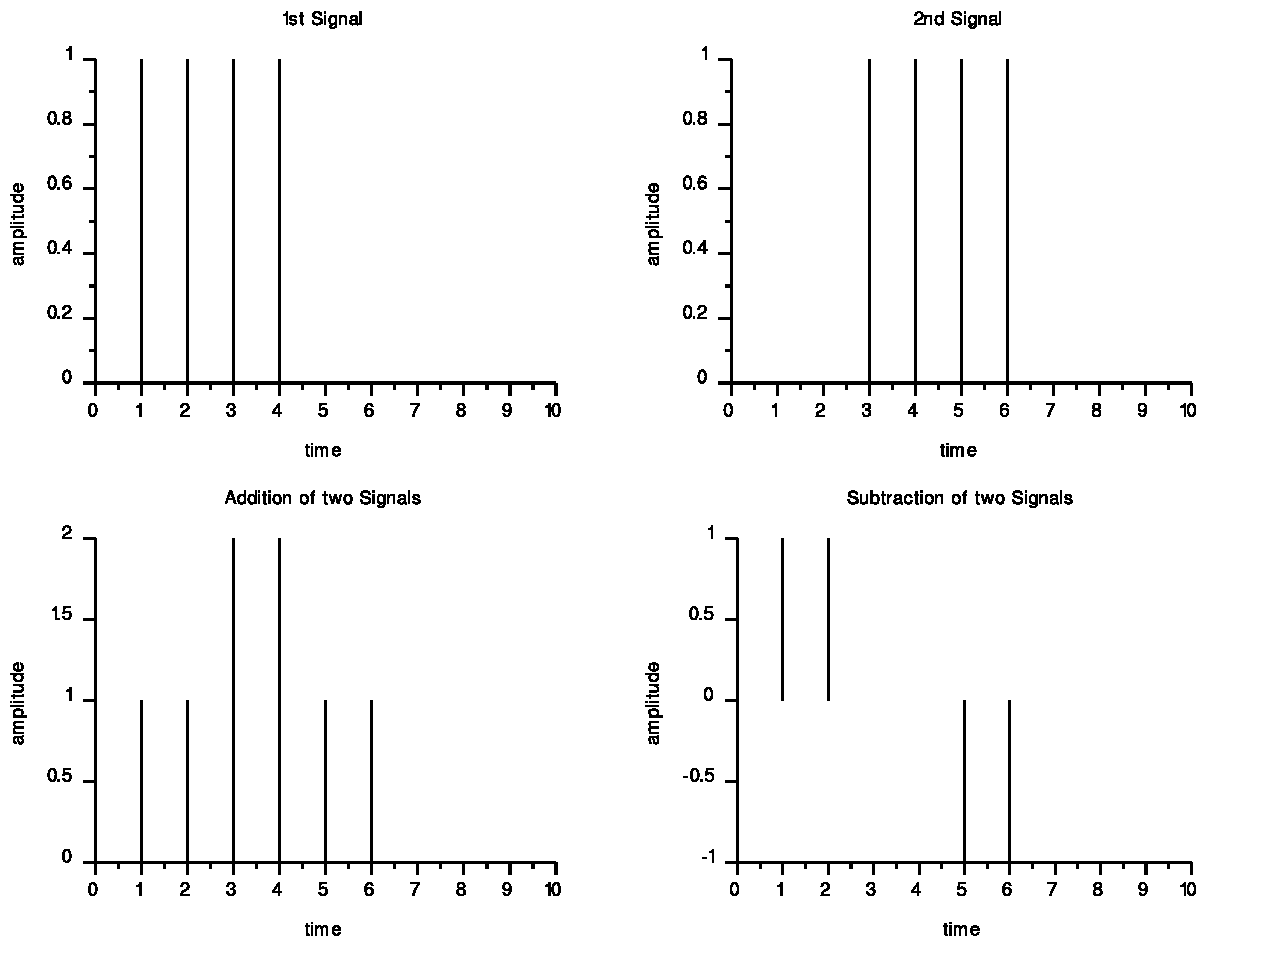
\includegraphics[scale=.5]{/home/kavya/kavyadev/DSPlab/scilabCode/addSubtract.pdf}
\caption{Plot of signals, their sum and their difference}
\label{addSub}
\end{figure}

\begin{figure}
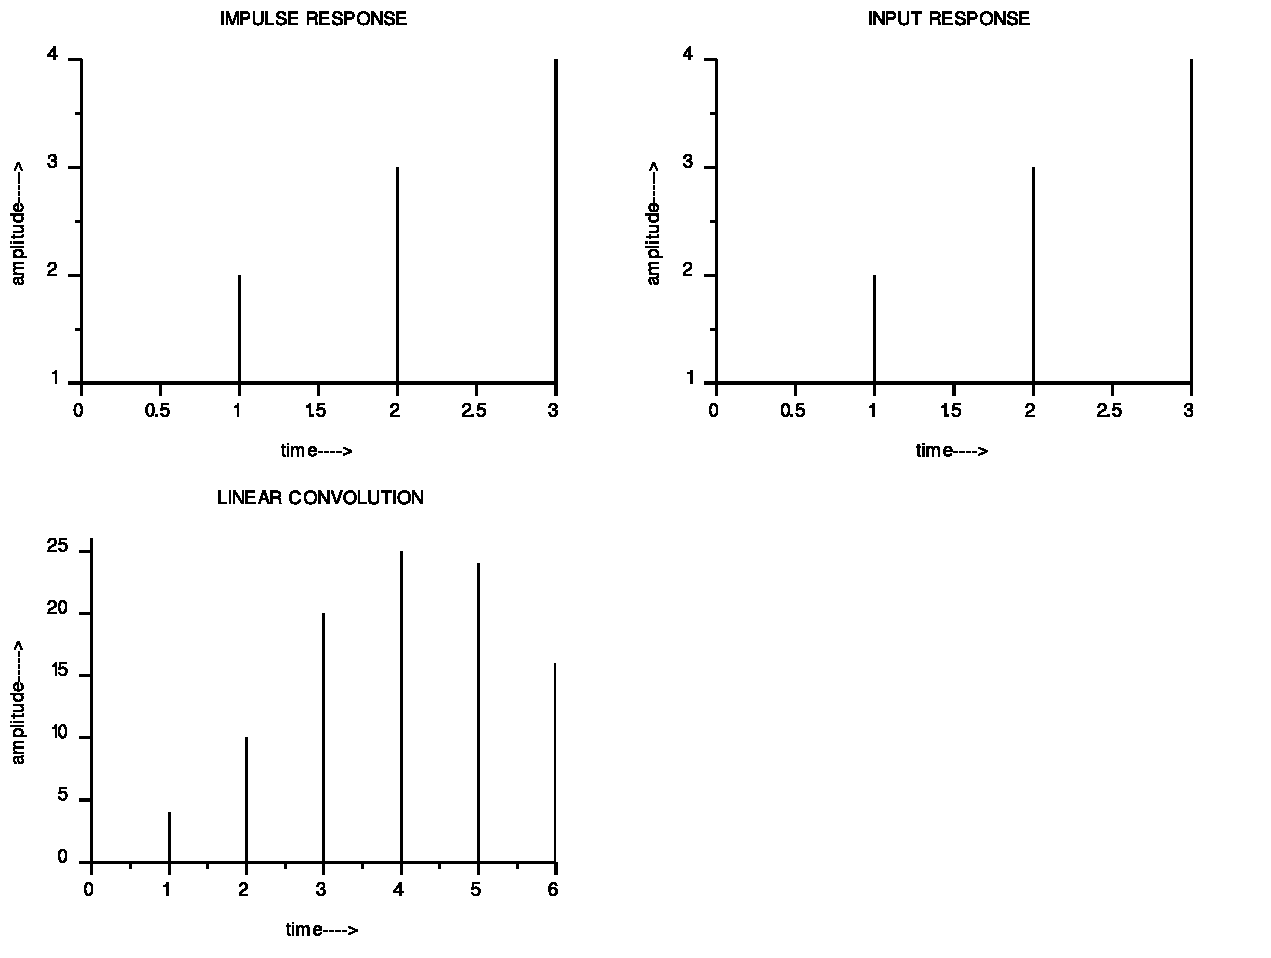
\includegraphics[scale=.5]{/home/kavya/kavyadev/DSPlab/scilabCode/linearconvolution.pdf}
\caption{Linear convolution of two sequences}
\label{linconv}
\end{figure}


